% Ensure that you compile using XeLaTeX !!! PDFTex has problems with some of the packages used
\documentclass[12pt]{article}
\setlength\parindent{0pt}

\usepackage{parskip}
\usepackage[margin=0.5in]{geometry}
\usepackage{fullpage}
\usepackage{moresize}
\usepackage{graphicx}
\usepackage{caption}
\usepackage{subcaption}
\usepackage{float}
\usepackage{xcolor}
\usepackage{soul}
\usepackage{fontspec}
\setmainfont{Doulos SIL}

\begin{document}

\begin{center}
\textbf{{\color{violet}{\HUGE 20201104 Wednesday\\}}}

\textbf{{\color{violet}{\HUGE ALL EXAMS (with notes)\\}}}

\end{center}
\newpage

\begin{center}
\textbf{{\color{blue}{\HUGE START OF EXAM\\}}}

\textbf{{\color{blue}{\HUGE Student ID: 44746\\}}}

\textbf{{\color{blue}{\HUGE 4:00\\}}}

\end{center}
\newpage

{\large Question 1}\\

Topic: Other (pre-midterm)\\
Source: Week 5 \& 6 Handouts\\

Explain how you could analyze this dataset in terms of sequential patterns vs. paradigmatic patterns.\\

\begin{figure}[H]
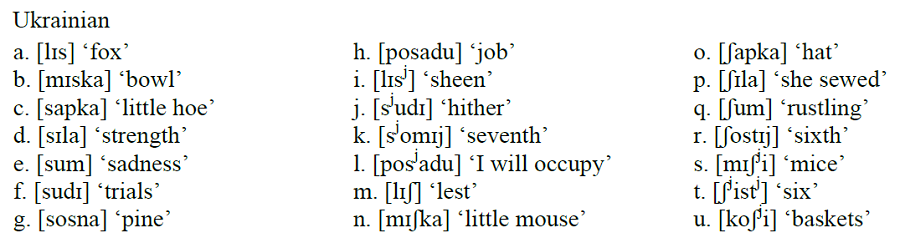
\includegraphics{../images/ukrainian.png}
\end{figure}

~\\
INSTRUCTOR NOTES: 


\vfill
Excellent (3) ~~~ Good (2.2) ~~~ Fair (1.7) ~~~ Poor (0)
\newpage

{\large Question 2}\\

Topic: Skewed Distributions\\
Source: Quiz 4, Question 1\\

L$_X$ (Language X) has three vowels, [i], [a], and [u]. It has bi-syllabic roots like Kikuyu. It does not allow non-identical high vowels to co-occur. Of the following nine logically possible vocalic sequences, which ones should be unattested in L$_X$? Explain why.\\

\begin{itemize} \item {[i...i]} \item {[i...a]} \item {[i...u]} \item {[a...i]} \item {[a...a]} \item {[a...u]} \item {[u...i]} \item {[u...a]} \item {[u...u]} \end{itemize}


~\\
INSTRUCTOR NOTES: [i...u], [u...i]


\vfill
Excellent (3) ~~~ Good (2.2) ~~~ Fair (1.7) ~~~ Poor (0)
\newpage

\begin{center}
\textbf{{\color{red}{\HUGE END OF EXAM}}}\\

\end{center}
\newpage

\begin{center}
\textbf{{\color{blue}{\HUGE START OF EXAM\\}}}

\textbf{{\color{blue}{\HUGE Student ID: 74752\\}}}

\textbf{{\color{blue}{\HUGE 4:10\\}}}

\end{center}
\newpage

{\large Question 1}\\

Topic: Skewed Distributions\\
Source: Week 5 Handout, Question 3\\

What evidence is there that there is a pattern in these data, assuming that these are the only CV and VC sequences that occur in some language?\\

{[sa]}, {[ʃi]}, {[za]}, {[ʒi]}, {[as]}, {[iʃ]}, {[az]}, {[iʒ]}


~\\
INSTRUCTOR NOTES: (the palatal sounds occur with the high vowel, while the alveolar sounds occur with the low vowel)


\vfill
Excellent (3) ~~~ Good (2.2) ~~~ Fair (1.7) ~~~ Poor (0)
\newpage

{\large Question 2}\\

Topic: Other (pre-midterm)\\
Source: Week 5 \& 6 Handouts\\

Explain how you could analyze this dataset in terms of sequential patterns vs. paradigmatic patterns.\\

\begin{figure}[H]
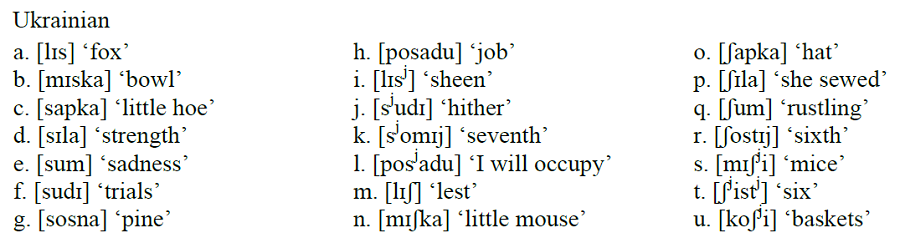
\includegraphics{../images/ukrainian.png}
\end{figure}

~\\
INSTRUCTOR NOTES: 


\vfill
Excellent (3) ~~~ Good (2.2) ~~~ Fair (1.7) ~~~ Poor (0)
\newpage

\begin{center}
\textbf{{\color{red}{\HUGE END OF EXAM}}}\\

\end{center}
\newpage

\begin{center}
\textbf{{\color{blue}{\HUGE START OF EXAM\\}}}

\textbf{{\color{blue}{\HUGE Student ID: 94263\\}}}

\textbf{{\color{blue}{\HUGE 4:20\\}}}

\end{center}
\newpage

{\large Question 1}\\

Topic: Articulatory Phonetics\\
Source: Homework 1, Question 3(a)\\

Could this image be the result of producing the sound represented by the given IPA symbol? Why or why not?\\

{[ɾ]}

\begin{figure}[H]
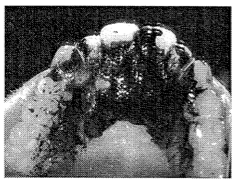
\includegraphics{../images/staticpalatography_stop.png}
\end{figure}

~\\
INSTRUCTOR NOTES: yes


\vfill
Excellent (3) ~~~ Good (2.2) ~~~ Fair (1.7) ~~~ Poor (0)
\newpage

{\large Question 2}\\

Topic: Phonological Features\\
Source: Quiz 3, Question 3\\

Explain why this featural specification either does or does not match the given sound.\\

{[-consonantal]}, {[+sonorant]}

{[h]}


~\\
INSTRUCTOR NOTES: does not match: [h] is [-cons] but also [-son], because its constriction is in the larynx, not the vocal tract


\vfill
Excellent (3) ~~~ Good (2.2) ~~~ Fair (1.7) ~~~ Poor (0)
\newpage

\begin{center}
\textbf{{\color{red}{\HUGE END OF EXAM}}}\\

\end{center}
\newpage

\begin{center}
\textbf{{\color{blue}{\HUGE START OF EXAM\\}}}

\textbf{{\color{blue}{\HUGE Student ID: 70875\\}}}

\textbf{{\color{blue}{\HUGE 4:30\\}}}

\end{center}
\newpage

{\large Question 1}\\

Topic: Articulatory Phonetics\\
Source: Week 3 Handout, Question 9\\

Explain how to figure out what the sound being produced is in this diagram.\\

\begin{figure}[H]
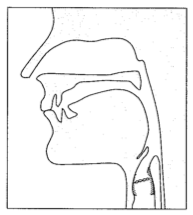
\includegraphics{../images/sagittal_m.png}
\end{figure}

~\\
INSTRUCTOR NOTES: [m] (check voicing, place, manner, and velum)


\vfill
Excellent (3) ~~~ Good (2.2) ~~~ Fair (1.7) ~~~ Poor (0)
\newpage

{\large Question 2}\\

Topic: Other (pre-midterm)\\
Source: Week 5 \& 6 Handouts\\

Explain how you could analyze this dataset in terms of sequential patterns vs. paradigmatic patterns.\\

\begin{figure}[H]
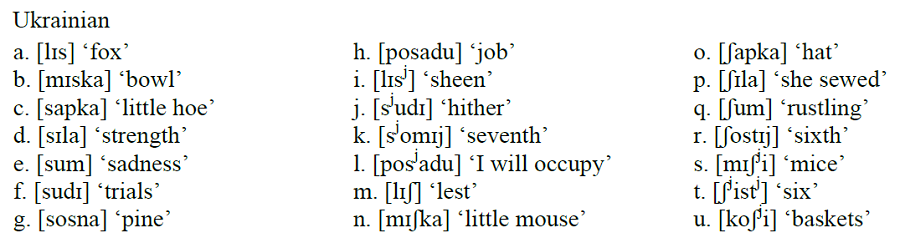
\includegraphics{../images/ukrainian.png}
\end{figure}

~\\
INSTRUCTOR NOTES: 


\vfill
Excellent (3) ~~~ Good (2.2) ~~~ Fair (1.7) ~~~ Poor (0)
\newpage

\begin{center}
\textbf{{\color{red}{\HUGE END OF EXAM}}}\\

\end{center}
\newpage

\begin{center}
\textbf{{\color{blue}{\HUGE START OF EXAM\\}}}

\textbf{{\color{blue}{\HUGE Student ID: 12377\\}}}

\textbf{{\color{blue}{\HUGE 4:40\\}}}

\end{center}
\newpage

{\large Question 1}\\

Topic: Phonological Features\\
Source: Week 4 Discussion\\

Explain why phonological features are used instead of phonetic characteristics in analyzing datasets.\\


~\\
INSTRUCTOR NOTES: Phonological features help to capture phonological patterns, i.e., they group sounds together based on whether they do things like triggering a change or undergoing a change. Phonological features are sometimes language-specific. Phonetic characteristics are simply descriptions of the physical properties of the sounds; they are language-universal and independent of the patterns (though it turns out that many phonological patterns are based on phonetic characteristic groupings).


\vfill
Excellent (3) ~~~ Good (2.2) ~~~ Fair (1.7) ~~~ Poor (0)
\newpage

{\large Question 2}\\

Topic: Other (pre-midterm)\\
Source: Week 4 Handout, Part II, Question 3\\

Explain how you would figure out what the Luiseño form is for the morpheme whose meaning is given below. (To be clear: you do NOT need to give me the form itself -- just explain the process of figuring it out.)\\

‘drink’

\begin{figure}[H]
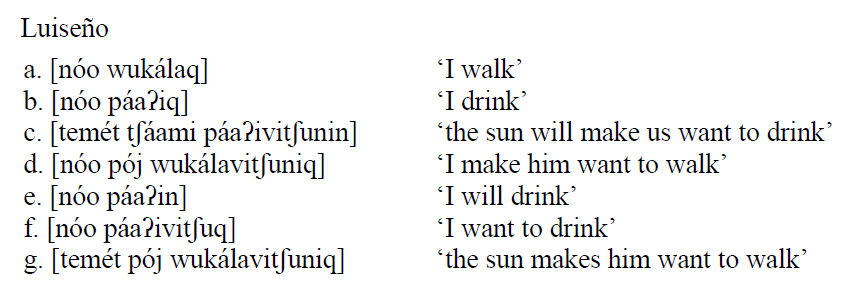
\includegraphics{../images/luiseno.png}
\end{figure}

~\\
INSTRUCTOR NOTES: ([páaʔi])


\vfill
Excellent (3) ~~~ Good (2.2) ~~~ Fair (1.7) ~~~ Poor (0)
\newpage

\begin{center}
\textbf{{\color{red}{\HUGE END OF EXAM}}}\\

\end{center}
\newpage

\begin{center}
\textbf{{\color{blue}{\HUGE START OF EXAM\\}}}

\textbf{{\color{blue}{\HUGE Student ID: 36593\\}}}

\textbf{{\color{blue}{\HUGE 4:50\\}}}

\end{center}
\newpage

{\large Question 1}\\

Topic: Phonological Features\\
Source: Week 4 Discussion\\

Explain what the given feature’s value is for this class of sounds, and why.\\

{[consonantal]}

glides


~\\
INSTRUCTOR NOTES: [-], because the constriction isn't as narrow as it would be for a fricative


\vfill
Excellent (3) ~~~ Good (2.2) ~~~ Fair (1.7) ~~~ Poor (0)
\newpage

{\large Question 2}\\

Topic: Skewed Distributions\\
Source: Week 5 Handout, Question 7\\

Explain how you would go about looking for co-occurrence restrictions in bi-syllabic signs in ASL. (Refer to the data that follows.)\\

\begin{figure}[H]
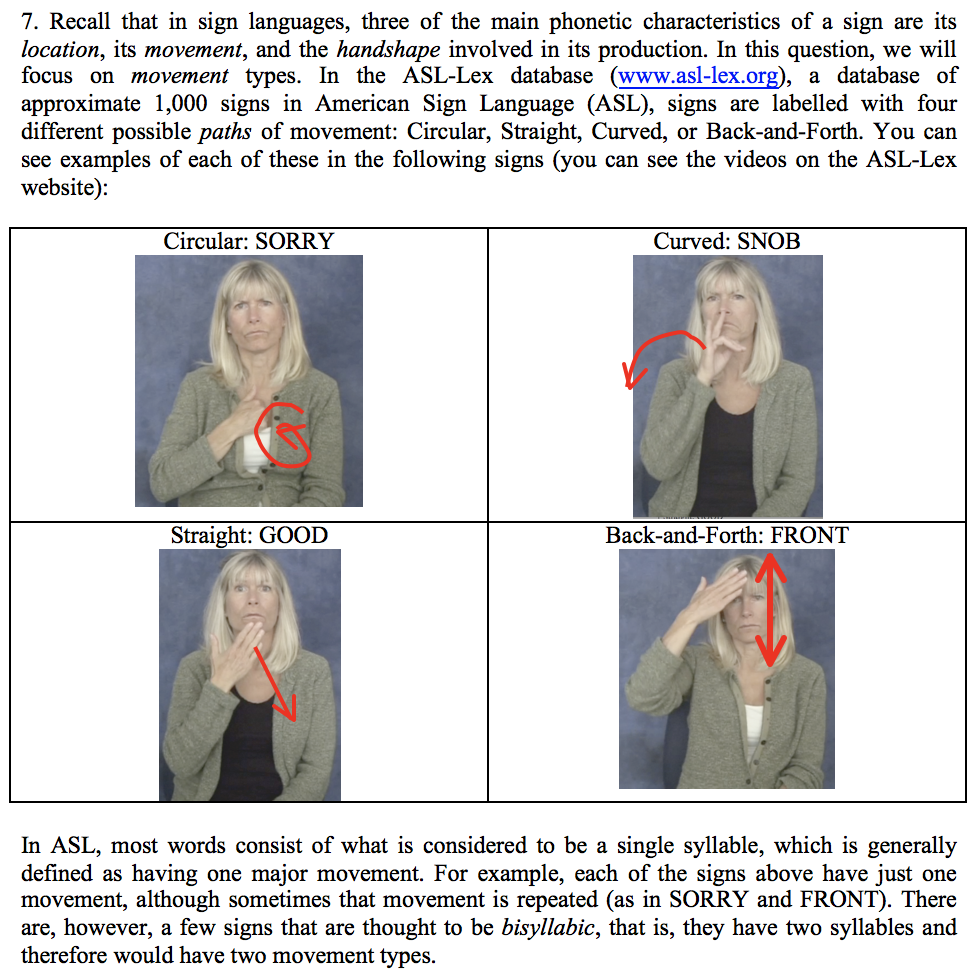
\includegraphics{../images/ASL_movement.png}
\end{figure}

~\\
INSTRUCTOR NOTES: You would start by coming up with all the possible combinations expected (i.e., 4x4 = 16). Then you'd compare that to some database of signs in ASL and see which combinations are actually attested or unattested.


\vfill
Excellent (3) ~~~ Good (2.2) ~~~ Fair (1.7) ~~~ Poor (0)
\newpage

\begin{center}
\textbf{{\color{red}{\HUGE END OF EXAM}}}\\

\end{center}
\newpage

\end{document}

